\documentclass[tikz,convert={density=800,outext=.png},border=5pt]{standalone}
%\documentclass[tikz, border=5pt]{standalone}

\usepackage[T2A]{fontenc}       			%поддержка кириллицы
\usepackage[utf8]{inputenc}					% Выбор языка и кодировки
\usepackage[english]{babel}
\usepackage{amsmath} % nice math symbols
     

\usepackage{tikz}
\usetikzlibrary{shapes,positioning,calc,patterns,decorations.pathreplacing}

\newcommand{\situation}[3]{
	\node[draw, circle, fill=white, scale=1.5] (sit_#1) at (#2pt,#3pt) {};
}
\begin{document}
	
	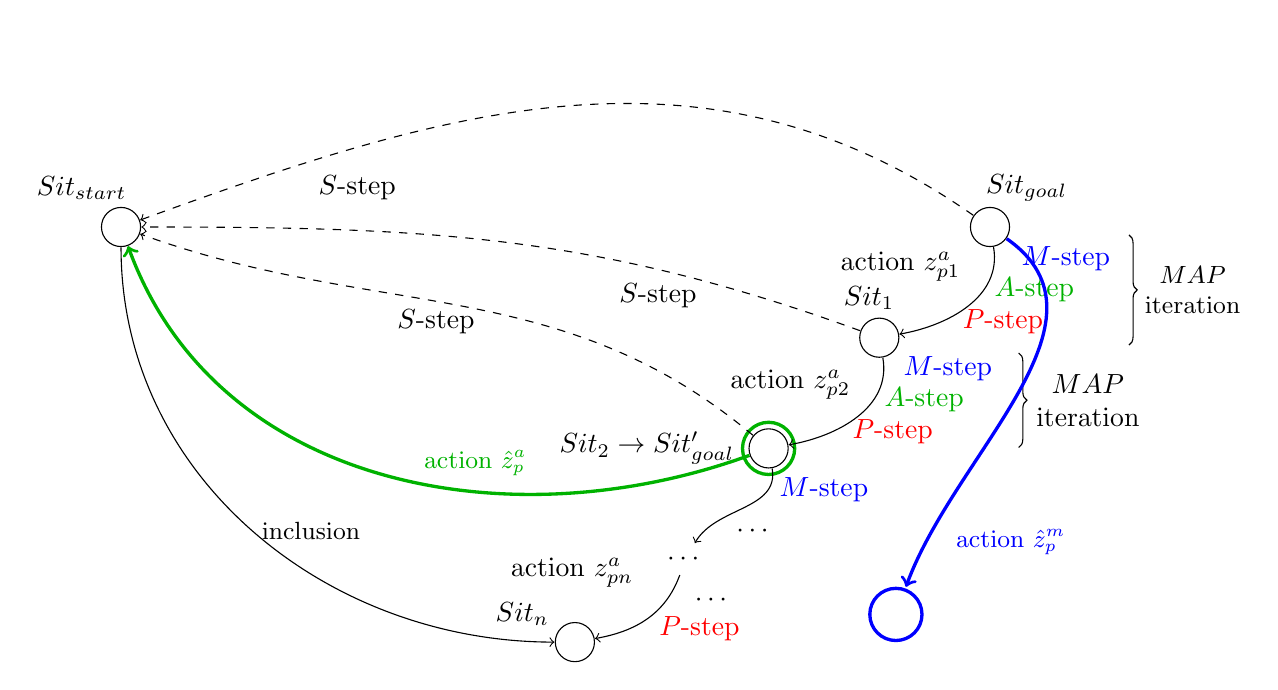
\begin{tikzpicture}
		\situation{st}{0}{0};
		\node[align=center] at (-0.5,0.5) {$Sit_{start}$};
		\situation{end}{314}{0};
		\node[align=center] at (11.5,0.5) {$Sit_{goal}$};
		
		
		\situation{1}{274}{-40};%114pt = 4cm
		\situation{2}{234}{-80};
		\node[draw, color=green!70!black, very thick, circle, scale=2] (sit_31) at (234pt,-80pt) {};		
		\node (all) at (204pt,-120pt) {$\cdots$};
		\situation{3}{164}{-150};
		
		\draw[->] (sit_end) to[out=-80,in=10] (sit_1);
		\draw[->] (sit_1) to[out=-80,in=10] (sit_2);
		\draw[->] (all) to[out=-110,in=10] (sit_3);
		
		\draw[->] (sit_2) to[out=-80,in=60] (all);
		
		\node at (9.9,-0.5) {action $z^a_{p1}$};
		\node[align=center, color=blue] at (12,-0.4) {$M$-step};
		\node[align=center, color=green!70!black] at (11.6,-0.8) {$A$-step};
		\node[align=center, color=red] at (11.2,-1.2) {$P$-step};
		\draw [decorate,decoration={brace,amplitude=3pt,mirror}]
		(12.8,-1.5) -- (12.8,-0.1) node[align=center,midway,font=\small,xshift=23pt] {$MAP$\\iteration};
		\node[align=center] at (9.5,-0.9) {$Sit_1$};
		
		\node at (8.5,-2) {action $z^a_{p2}$};
		\node[align=center, color=blue] at (10.5,-1.8) {$M$-step};
		\node[align=center, color=green!70!black] at (10.2,-2.2) {$A$-step};
		\node[align=center, color=red] at (9.8,-2.6) {$P$-step};
		\draw [decorate,decoration={brace,amplitude=3pt,mirror}]
		(11.4,-2.8) -- (11.4,-1.6) node[align=center,midway,xshift=25pt] {$MAP$\\iteration};		
		\node[align=center] at (190pt,-80pt) {$Sit_2\rightarrow Sit'_{goal}$};

		\node[align=center, color=blue] at (254pt,-95pt) {$M$-step};
		\node[align=center] at (229pt,-110pt) {$\cdots$};

		\node[align=center] at (214pt,-135pt) {$\cdots$};
		\node[align=center, color=red] at (209pt,-145pt) {$P$-step};
		\node at (163pt,-125pt) {action $z^a_{pn}$};
		\node[align=center] at (145pt,-140pt) {$Sit_n$};

		\draw[->,color=green!70!black, very thick] (sit_2) to[out=-160, in = -70] (sit_st);
		\node[font=\small,color=green!70!black] at (4.5, -3) {action $\hat z^a_p$};
		

		
		\draw[<-] (sit_3) to[out=-180, in = -90] node[font=\small,right]{inclusion} (sit_st);
		
		\draw[->,dashed] (sit_2) to[out=140,in=-20] (sit_st);
		\node[align=center] at (194pt,-25pt) {$S$-step};
		\draw[->,dashed] (sit_end) to[out=145, in = 20] (sit_st);
		\node[align=center] at (3,0.5) {$S$-step};
		\draw[->,dashed] (sit_1) to[out=160, in = 0] (sit_st);
		\node[align=center] at (4,-1.2) {$S$-step};
		
		
		\node[draw, color=blue, very thick, circle, scale=2] (sit_ng) at (280pt,-140pt) {};
		\draw[->,color=blue, very thick] (sit_end) to[out=-35, in = 70] (sit_ng);
		\node[font=\small,color=blue] at (11.3, -4) {action $\hat z^m_p$};
	\end{tikzpicture}


\end{document}